\section*{Introduction}
Ce TP est un exemple de manipulation de RMI.

\section*{Listing des dossiers et fichiers du projet}
\begin{description}
	\item[doc/ :] javadoc du projet
	\item[lib/ :] contient les librairies (\verb+.jar+) dont le projet est dépendant
	\item[src/ :] contient les fichiers sources (\verb+.java+) du projet
	\item[test/ :] contient les fichiers de tests
	\item[uml/ :] contient les diagrammes de classes du projet
	\item[build.xml :] fichier de gestion de projet Ant
	\item[client.jar :] archive exécutable du client
	\item[java.policy :]
	\item[rmi.eps :] schéma général de rmi
	\item[runclient.sh :] script de lancement d'un client
	\item[runserver.sh :] script de lancement d'un serveur
	\item[server.jar :] archive exécutable du serveur
	\item[sonar-project.properties :] fichier .properties pour le contrôle qualité Sonar
\end{description}

\section*{Utilisation}
	\underline{Noeud serveur}\\
		java -Djava.security.policy=java.policy -jar server.jar [-tree|-graph] <id\_noeud>\\
	\underline{Client}\\
		java -Djava.security.policy=java.policy -jar client.jar <fichier\_conf> <nom\_pc\_distant> <message>
	
			
\section*{Architecture}
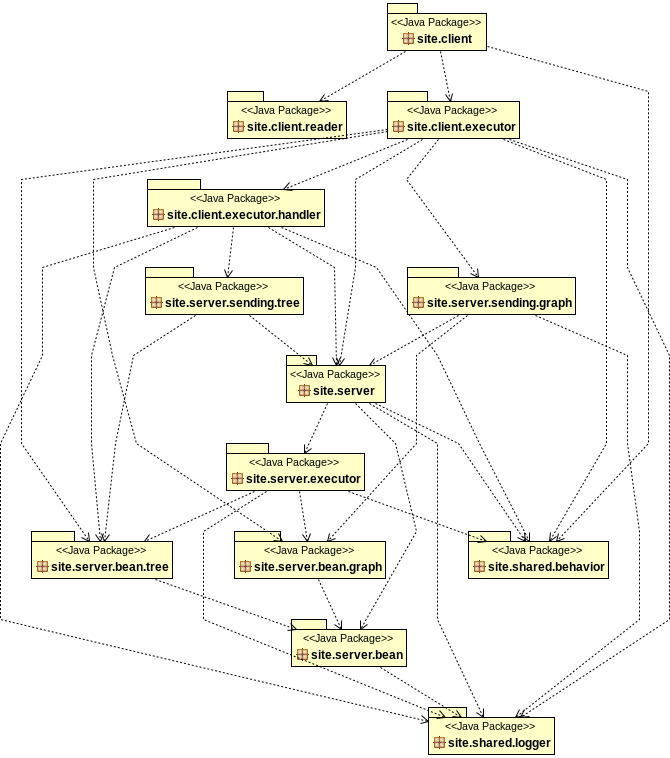
\includegraphics[width=\textwidth]{../uml/overview.png}
\newpage
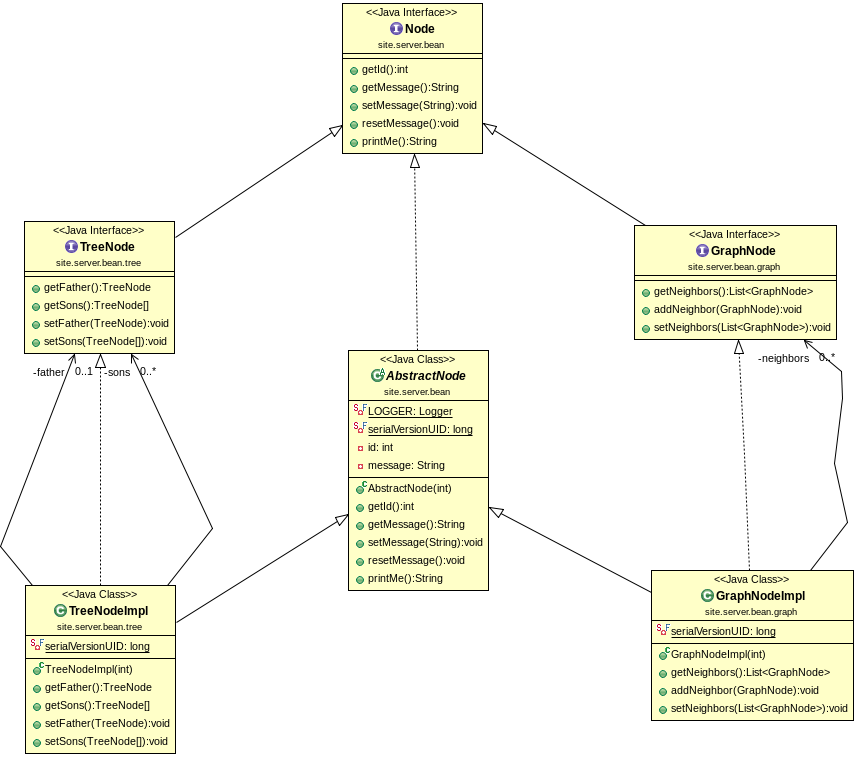
\includegraphics[width=\textwidth]{../uml/bean.png}
\newpage
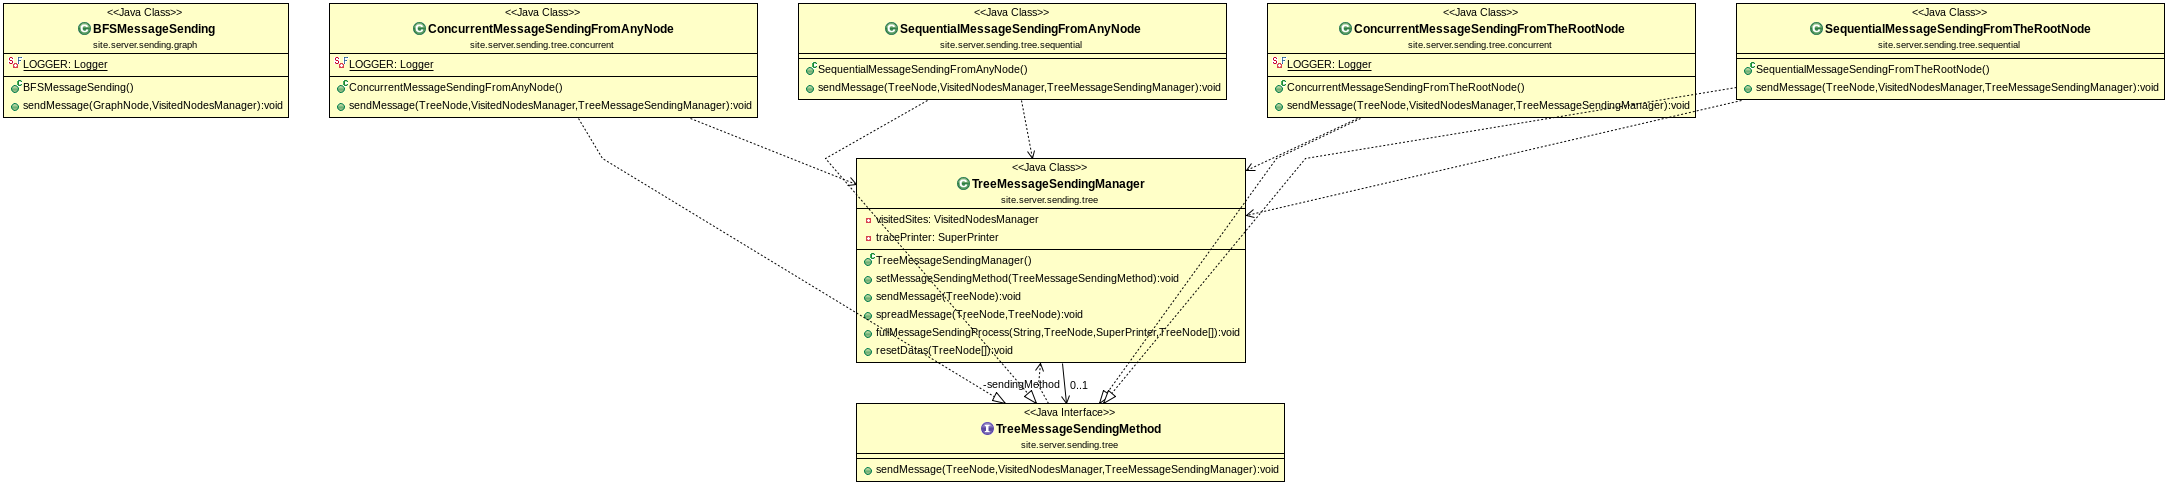
\includegraphics[width=\textwidth]{../uml/sending.png}
\\~\\
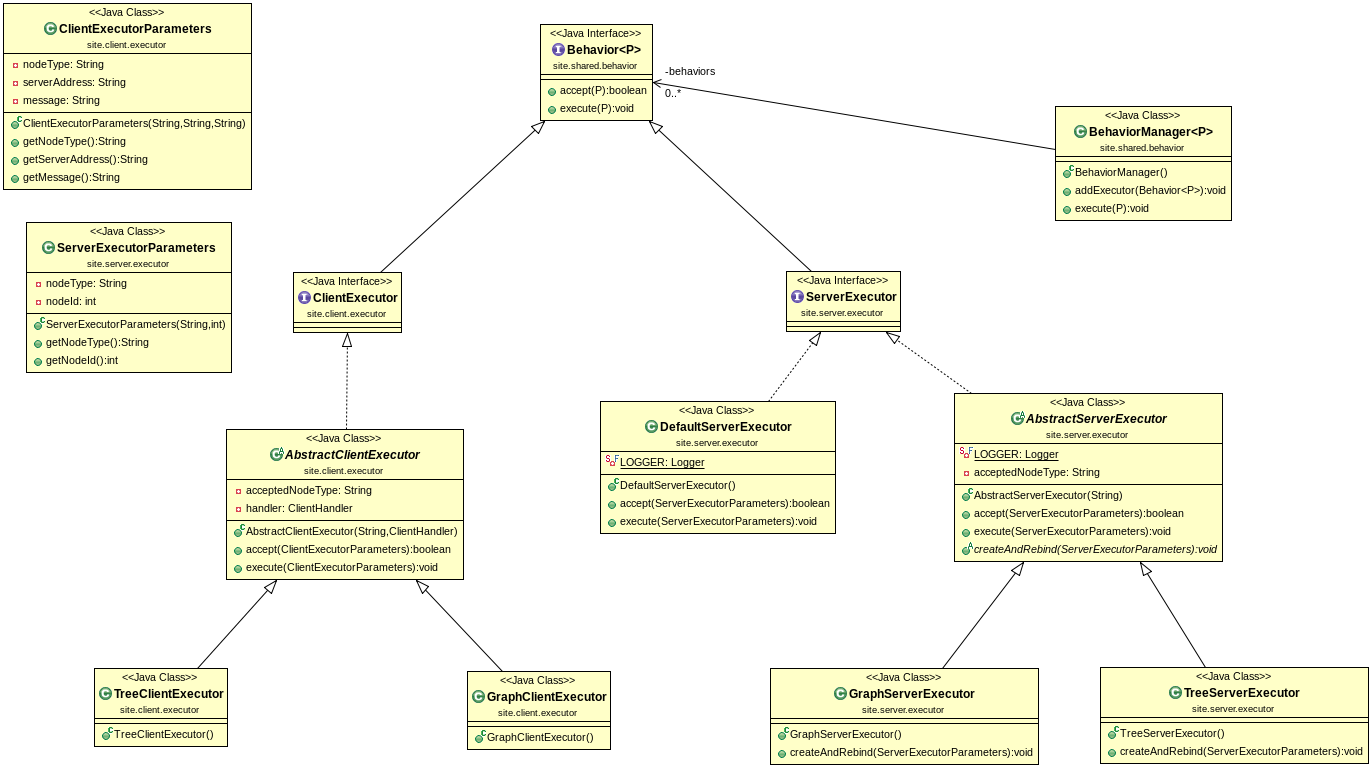
\includegraphics[width=\textwidth]{../uml/behavior.png}

